\chapter{DIMENSIONAMIENTO DE LARGUERO PRINCIPAL (RIEL)}

\section{Selección de material y/o perfil.} % section headings are printed smaller than chapter names
\makebox[\textwidth]{AISI 1045} \par
Este es un perfil sólido que se encuentra en cualquier distribuidora de metales, el cual se puede comprar por perfil y son bastante largos. Este perfil lo teníamos a nuestro alcance gracias a que un integrante del equipo lo donó para el trabajo, al observar sus características, observamos que cumple con el diseño y gracias a que es un material dúctil, no tanto como el aluminio, se puede observar la deformación .
\\\

\section{Esfuerzo y deformación máxima, (DMF y DEC).}

\begin{table}[htb]
\centering

\begin{tabular}{| p{2.8cm}| p{2.8cm} |}
\hline
\multicolumn{2}{|c|}{AISI 1045} \\
\hline
E &  $\sigma$y \\
\hline \hline
600 MPa & 190-205 GPa  \\ \hline
\end{tabular}
\caption{Propiedades mecánicas}
\label{}
\end{table}

\begin{center}
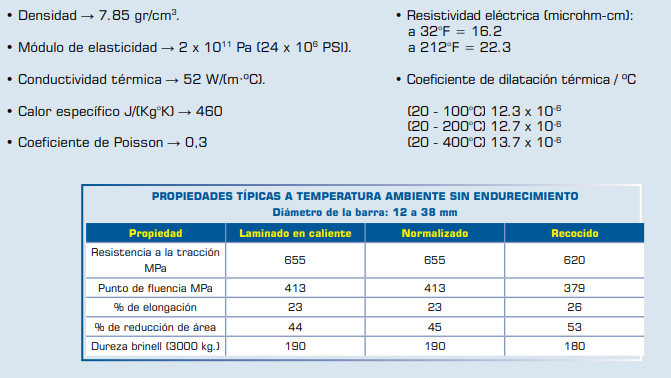
\includegraphics[width=.6\linewidth]{B/figs/B_1.png} 
\end{center}


\subsection{Cargas de diseño}


\begin{equation*}
\textrm{ Polipasto } = 0 .8 \textrm{ Kg}
\end{equation*}
\begin{equation*}
\textrm{ Transmisión} = 0.4 \textrm{ Kg}
\end{equation*}
\begin{equation*}
\textrm{ Elementos para carga } = 5.3 \textrm{ Kg}
\end{equation*}

\subsection{Cálculos de la viga} 

\begin{center}
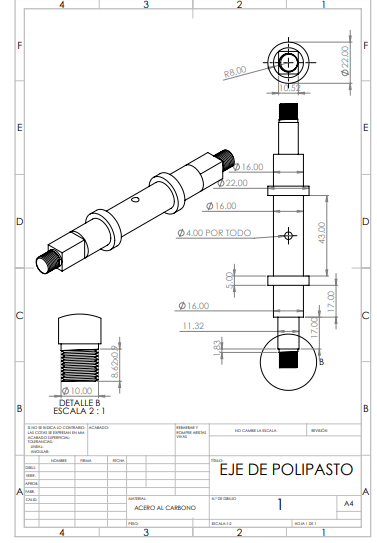
\includegraphics[width=1\linewidth]{B/figs/C_1.png} 
\end{center}



\begin{align*}
\sigma y & = \frac{M C}{I} \\
        & = \frac{18.11 * 1.58X10^{-3}}{\frac{(0.03175 *  3.17X10^{-3})^{3}}{12}} \\
        & = 339.49 \textrm{ MPa}\\
\end{align*}


\textrm{ con este cálculo se eligió el material que soportará un esfuerzo con un factor}\\ 
\textrm{ de seguridad de}
  
  \begin{align*}
   F.S. & = \frac{600x10^{9}}{339.49} = 1.76 \\
\end{align*}


\begin{center}
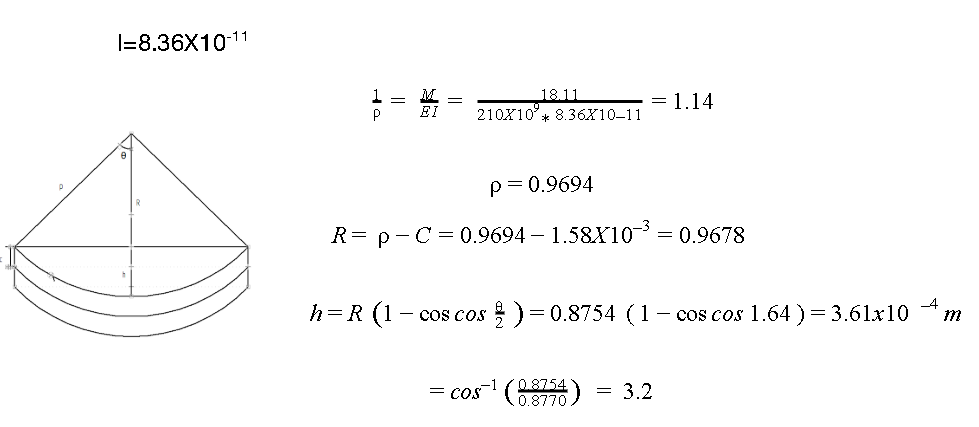
\includegraphics[width=1\linewidth]{B/figs/C_21.png} 
\end{center}

